% Some commands used in this file
\newcommand{\package}{\emph}

\chapter{Introduction}
Compilers are complex pieces of software that transform source code written in a high-level language into target-specific machine code while optimizing the output for performance on the target machine. Besides the compiler itself often being a large open-source project containing thousands of lines of code, the transformations applied by compiler optimization passes range from small, local optimizations to more aggressive rewrites that optimize the code in more intrusive ways.
While such optimizations improve the performance of the generated machine code, if applied incorrectly, they can lead to bug densebgy machine code that does not adhere to the semantics intended in the original source code. Compiler bugs steem from mistakes in the implementation of the compiler itself or can be introdcued due to the lack of clear defined sematics for both the source and target languages can lead to differing interpretations of what constitutes correct machine code generation, resulting in inconsistencies.

Nevertheless compiler are one of the most important pieces of software and there have been various research efforts that implemented fully verified compiler infrastructures which provide correctness guarantees for their produced output programs. Since these compiker often over cover a subset f langaes and are support less optimizaton compared their non-verfied counterparts they are not the dayto day compiler s of producion systems and additionally are often independent projects.

LLVM, the low-level virtual machine open source compiler project is compiler infrastrucutre framework which is used inside compiler of many programming languages such as the Rust or Lean compiler. LLVM hasa huge opensource codebase consnsiting of thousand of lines of code. Additionally at the core of  LLVM is also its LLVM IR  that is an intermeidate representation that the reuse optimization and perform optimizations independtn of the source programming language by lowering to LLVM IR. This allows LLVM to be easily reused for new compilers since only a new frontend needs to be provdied while the rest of the pipeline can leverage the llvm toolchain.
Given the size of the LLVM compile rtoolchain formally verificartin of the conpiler is unlikely. Still a bug in llvm can affect the compilatuon of various programmingl nagugaes given llvm's design. Additioany LLVM is used in compilers for varois programming lnaguaes like Rust and Lean. having formal guarantees for LLVM transforamtions would be attrative for Lean, whch is a theorem prover and uses its compler to provided proof certifactes. A compiler bug in LLVM can here therefore affect the validity of proof certifctes.   The rust compiler also uses LLVM within the standart complation path and many projects focus on providng guaranteed  on the level of rust language itself as soon as the program is lowered to LLVM IR, the trustwortghyness hinges on the thrustworthyness of the llvm toolchain. 

Whle recent research efforts focus on the higher lelve llvm stack and projects like Alive2 prform translation validation for LLVM IR transformations, the llvm backends have received less attention .

Therefore to counteract this gap and motivated by brining formal verifcation tto the llvm ecosystem this thesis implementes a pass to apply verified instruction selection from   for a subset of arithemtic instruction LLVM IR to Riscv-64, where the instruction selection from LLVM IR to Risc-V  provides formal correctness guarantees in the Lean theorem prover. We will introduce an instruction selection pipeline that lowers LLVM IR, assuming certain constraints on the LLVM program shape, and translates it to RISC-V. This transformation is then guaranteed to be semantics-preserving, ensuring that the generated machine code faithfully implements the original LLVM IR logic and is implemented in the Lean theorem prover. To guarantee rigorous semantics and avoid inconsistencies, we base our Risc-V semantics on the offical Risc-V ISA specifciation  and mechanization in Sail. 

We will focus on the arithemtic subset of LLVM-IR instructions containing bitwise operations and integer arithmetic.

By additionally proposing a verified peephole optimization pass for the generated RISC-V machine code, we introduce verfified assembly level optimizations in our work. Peephole optimizations are small, local transformations that improve performance or reduce code size without altering semantics. The motivation behind implementing an additional peephole rewriting pass is to reduce pathologies introdcued by the low-level instruction selection. Moreover, optimizing on the assembly level allows us to exploit architectural ISA-specific optimizations unavaible at the IR level.

The base of this work is the Lean-MLIR project, which provides a framework Lean-MLIR(X) for modelling SSA-based compiler IRs and their rewrites in an MLIR dialect style. SSA is an IR type where each variable is only assigned once and thereby has a unique point where it receives its value. MLIR is a compiler framework within the LLVM ecosystem that supports a hybrid IR consisting of many users defined domain-specific, tailored IR’s (dialects) within one framework.[to do section] (MLIR allows to build reusable and extensible compiler infrastructure that makes it easier to build domain-specifc compilers (e.g for specific hardware or a specifc domain) but also simplifies connecting existing compilers together.)


We will use and model a Risc-V as well as LLVM IR dialect to formalize and verify our instruction selection within the LeanMLIR(X) framework. The Lean-MLIR project also provides a semantic model for the arithmetic fragment of LLVM,  which will be used as the semantic model for LLVM IR.  For our Risc-V semantics, we rely on the formal specification provided by the Sail project and eextract it to implement the Risc-V semantics of our lowering. Sail is a domain-specific language (DSL) used to formalize ISA specifications and allows for their extraction into theorem provers. Therefore, Sail makes the semantics of an ISA directly accessible and usable from within a proof assistant. To implement the peephole rewriting pass, we draw from peephole optimization patterns used in LLVM backend and IR optimization passes like InstCombine and DAGCombine.

For verification, we aim to leverage Lean’s native support for bitvector reasoning and its integration of bv\_decide, the first fully verified SMT solver embedded in a theorem prover. Compared to other projects like CompCert, we try to implemnt our pipline to give us significantly more automation when reasoning about bit-level computations. 

By proving a verified instruction selection pass and a assembly peephole rewritting pass to be applied on LLVM IR code in its dialect form, we propose a way of incoperating trustworthy code generation from LLVM IR. When a developer does not want to trust the complex llvm ir backeends to lower the code, this pass shoudl give support and enable to lower it to machine code with formal correctness guarantees. Making it explicit what is hidden in the LLVM backends behind multiple stages. In addition, we allow our instruction selection pass to be visulaized in the command line using the implemetning the  well-know opt tool for LLVM and other xcompilers within Lean. This allows to compare the output of our pipeline with other tools. 




The contributions of this thesis are the following:

-Design and implement a verified instruction selection pass from LLVM IR (pure arithemtic fragment) to RISC-V machine code with proofs formalized in the Lean theorem prover.

-Develop a verified peephole optimization pass for the resulting RISC-V machine code

-Leverage existing semantic models and verified solvers and tactics in Lean to automate proof obligations

- Extended LeanMLIR to enable LLVM IR to assembly code verification.














There have been various academic and industrial efforts to implement formally verified compiler infrastructures and to validate or provide correctness guarantees for code lowerings, state-of-the-art compiler projects like LLVM, an open-source compiler framework with a wide range of optimization capabilities,  are large and complex. This makes full formal verification of their entire codebase highly challenging and impractical.


LLVM desgin's using a intermediate represenation allows any programming language to use its tools and a bug in the LLVM compiler stack can affect the compilation of many different source languages.

Lean, a functional programming language and interactive theorem prover which provides users with tools for formal verification and software development, leverages the LLVM toolchain as one of its backends. 

A Lean program is first lowered to Lean’s core language— a minimal representation suitable for verification by the Lean kernel. Then the  Lean code is translated to C and compiled using a C compiler such as Clang, which is built upon the LLVM toolchain.

\begin{figure}[htbp]
  \centering
  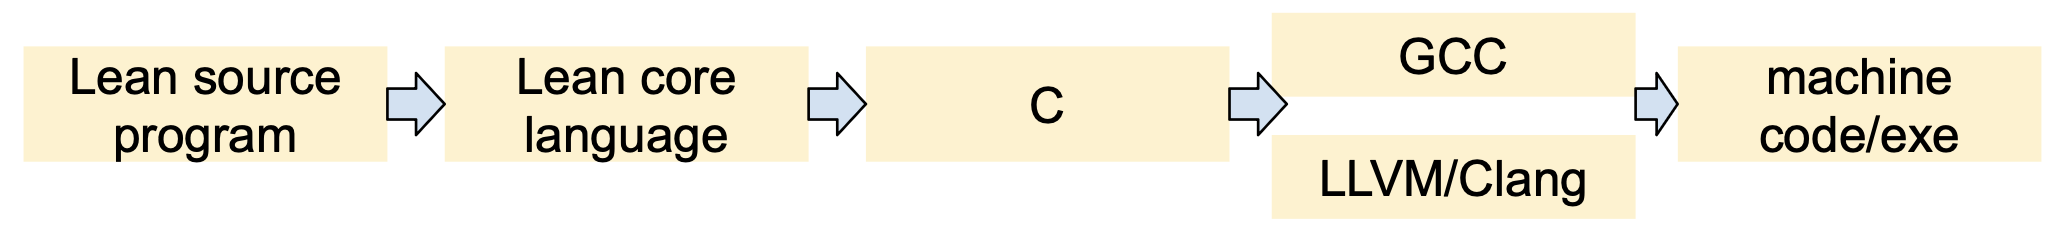
\includegraphics[scale=0.37]{thesis/Lean_Compilation_Pipeline.png}
 
  \caption{Lean compilation flow leveraging C compilers}
  \label{fig:your-label}
\end{figure}

This compilation path allows Lean programs to benefit from the mature optimizations provided by LLVM, but it also extends the trust boundary to include the external compiler infrastructure. Verifying the correctness of Lean’s compilation pipeline would therefore require verifying the entire Clang/LLVM stack.
However, in a setting of a theorem prover formallly verified compilation is desriable since miscompilation and bugs can lead to serious consequences that affect the soundness of the system. 

For example, the Lean compiler is crucial in a style of proof called 'proof by reflection', where a computation is executed, and the output of the computation is used as a proof certificate. Instead of constructing proof terms manually through deductive reasoning, proof by reflection uses computation to decide whether a proposition holds. The computation result is then reflected back into the proof to complete the original proof goal without re-executing the performed computation.  Therefore, if the computation output is incorrect (e.g., due to a miscompilation bug), a logically unsound proof term can be integrated into a proof, and the theorem prover will accept an unsound proof. In addition, there are proof strategies in Lean (native decide), where we explicitly trust the compiler to finish a proof goal, hence miscompilation there would finish a wrong proof. 
// to do : insert a proof goal where native decide is used. 

Therefore, trustworthy compilation and code generation for the LLVM compiler, which is used trustingly in settings like the Lean Theorem prover, is a relevant research target. At the time of this thesis there exist verification efforts that target the LLVM ecosystem and LLVM IR e.g. the Alive2 project, which verifies optimizations employed in the LLVM InstCombine pass, an IR-to-IR optimizations pass. Existing projects mostly focus on properties of the higher-level LLVM stack and rewrites within LLVM IR itself and do not focus on the LLVM backends. Meanwhile backends and low-level assembly code transformation are known to be the most bug dense compiler components. (quote peek paper). 

Therefore, to contribute to this space, we propose to take a subset of LLVM IR and write a formally verified backend component to produce machine code style SSA code. We will implement an instruction selection pipeline that lowers LLVM IR, assuming certain constraints on the LLVM program shape, and translates it to RISC-V. This   transformation is then guaranteed to be semantics-preserving, ensuring that the generated machine code faithfully implements the original LLVM IR logic. To guarantee rigorous semantics and avoid inconsistencies, this work bases its machine language semantics on the official RISC-V ISA specification.  

We will focus on the subset of LLVM-IR instructions that would typically be generated by Lean’s core language - primary bitwise operations and integer arithmetic, where we exclude stores. 

Additionally, we propose to build a verified peephole optimization pass for the generated RISC-V machine code, that implements optimizations used in production compilers like GCC and LLVM.  Peephole optimizations are small, local transformations that improve performance or reduce code size without altering semantics. The motivation behind implementing an additional peephole rewriting pass is to reduce inefficiencies that can be introduced during instruction selection. Moreover, optimizing on the assembly level allows us to exploit architectural ISA-specific optimizations.





\textbf{Organization of the thesis }

We started by explaining the necessity of verfified compiler infrastrcutrues and the use cse for the Lean theorem prover. Next we dive into the research fields of formally verified compiler components, optimization validitation, peephole optimizations, and semantics of LLVM IR and ISA's. Then the background chapter explores the essential topics to understand the design and tools used to implement our instruction selection and mechanization in the Lean theorem. Then we provide a high-level design overview of the instruction selection and peephole optimization pipeline. Then we explain the necessary steps in the implementation of our pipeline. Finally we evaluate the output of our instruction selection ad discuss possibilities to enhance our pipelie, 
